\section{\Large PROBLEM SET 4}
\subsection{PROBLEM 1}
\textit{Equilibrium tests}

\textit{a. Assume that 2 components of the initial angular velocities are zero and that the principal axes are aligned with the inertial frame (e.g., zero Euler angles). Verify that during the simulation the 2 components of angular velocity remain zero and that the attitude represents a pure rotation about the rotation axis (e.g., linearly increasing Euler angle). Plot velocities and angles.}

For this problem, we assumed that the initial angular velocity and Euler angles were what is shown below. The initial Euler angles were not initialized to be all 0 because we used 3-1-3 Euler angle representation, meaning that Euler angles at 0 would lead to a singularity. While this work-around is not ideal in the situation that the satellite operates around zero Euler angles, for the sake of this exercise this should be adequate.
\begin{align*}
\Vec{\omega} &= 
\qty[parse-numbers = false]{
    \begin{bmatrix}
    0 \\
    0 \\
    1 \\ 
    \end{bmatrix}
}{\radian\per\s}
\end{align*}
\begin{align*}
\phi = \qty[parse-numbers = false]{0}{\radian}, \;\;\;
\theta = \qty[parse-numbers = false]{1e-9}{\radian}, \;\;\;
\psi = \qty[parse-numbers = false]{0}{\radian}
\end{align*}

As can be seen in Figure \ref{fig:ps4_problem1a_velocity}, $\omega_x$ and $\omega_y$ remained 0, while $\omega_z$ was a constant value, as expected. Similarly, in Figure \ref{fig:ps4_problem1a_angle} the $\phi$ and $\theta$ Euler angles stayed zero while the $\psi$ Euler angle varied. 

\begin{figure}[H]
\centering
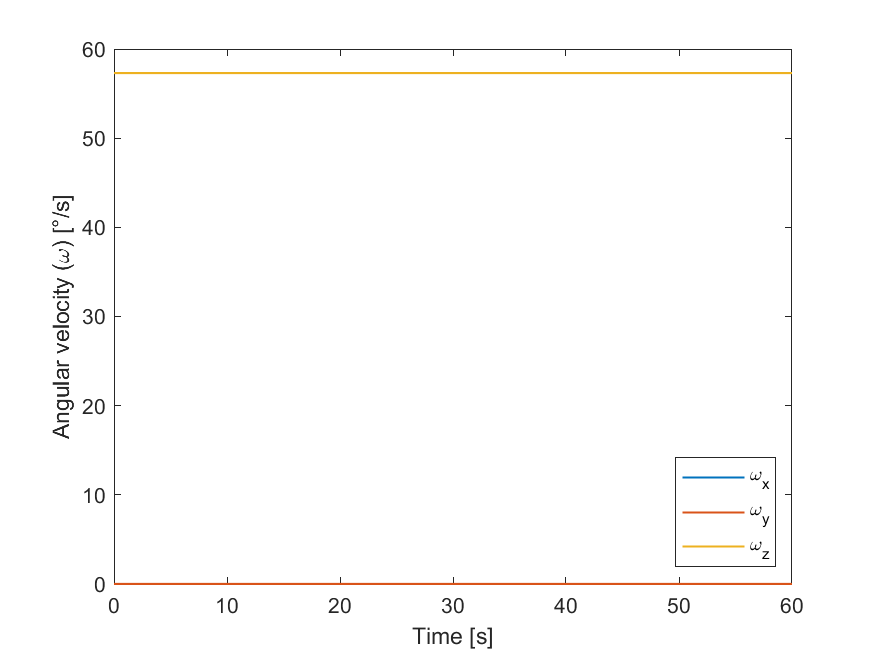
\includegraphics[scale=0.6]{Images/ps4_problem1a_velocity.png}
\caption{Evolution of angular velocity}
\label{fig:ps4_problem1a_velocity}
\end{figure}

\begin{figure}[H]
\centering
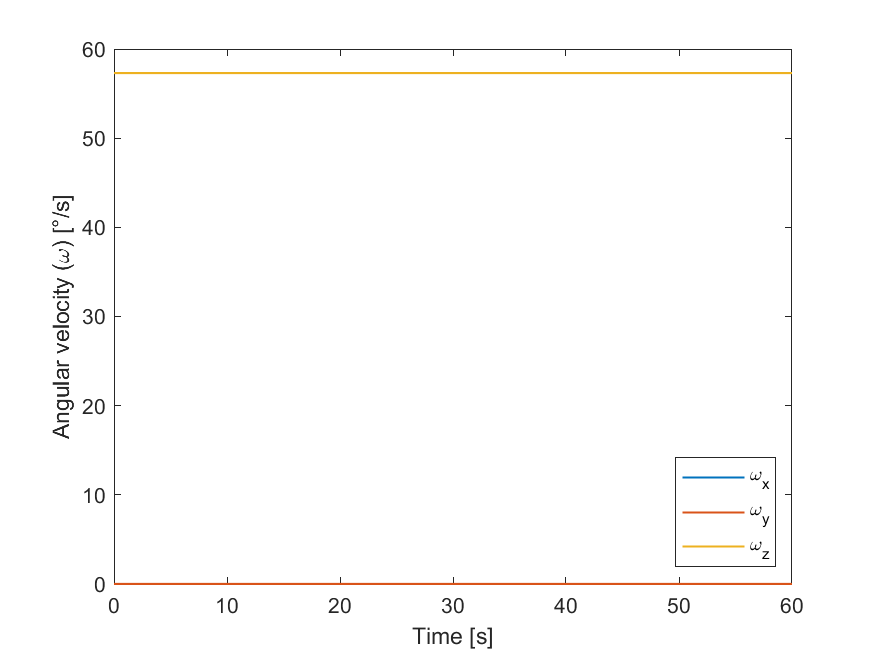
\includegraphics[scale=0.6]{Images/ps4_problem1a_angle.png}
\caption{Evolution of Euler angles}
\label{fig:ps4_problem1a_angle}
\end{figure}

\textit{b. Repeat a. by setting the initial attitude to match the RTN frame. Set the initial angular velocity to be non-zero only about N. Show the evolution of attitude motion in the RTN frame and give an interpretation of the results (recall that you might have J2 effects in orbit propagation, consider removing them for verification).}

\subsection{PROBLEM 2}
\textit{Stability tests}

\textit{a. Pretend you have a single-spin satellite. Set initial conditions to correspond alternatively to the 3 possible equilibrium configurations (rotation about principal axes of inertia). Slightly perturb initial condition. Is the attitude stable or unstable? In angles and velocities? If stable, periodically or asymptotically? Show it.}

For a single spin satellite, the three possible equilibrium configurations are spinning on its minimum principal axis, spinning on its intermediate principal axis, and spinning on its
maximum principal axis. Figures \ref{fig:ps4_problem2a_1}, \ref{fig:ps4_problem2a_2}, \ref{fig:ps4_problem2a_3}, all show that the Euler angles are relatively unstable in all of the cases. However, the angular velocities are periodically stable when spinning along the minimum and maximum axes and unstable when spinning on the intermediate axis.

\begin{figure}[H]
\centering
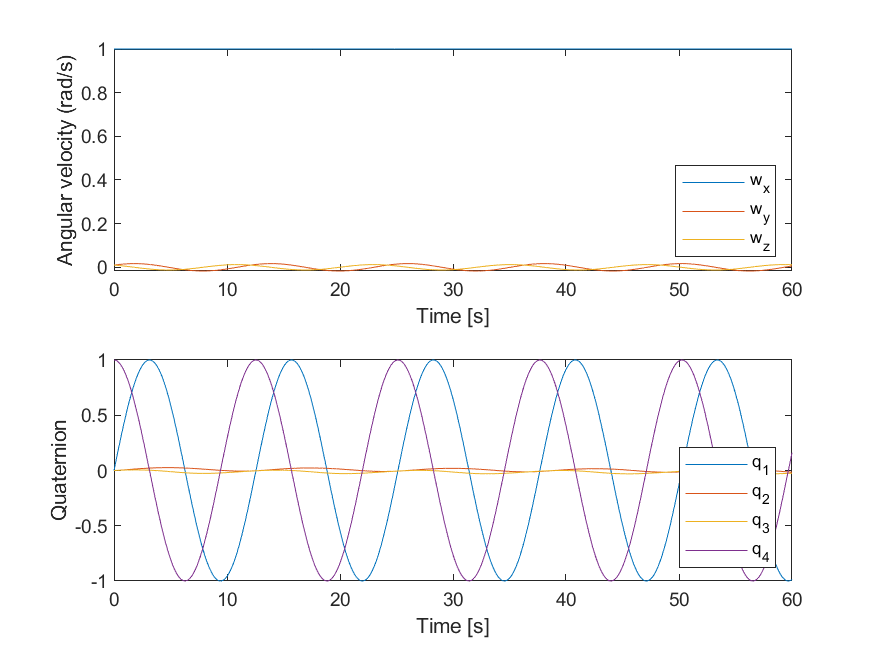
\includegraphics[scale=0.6]{Images/ps4_problem2a_1.png}
\caption{Simulation of satellite spinning on its minimum principal axis}
\label{fig:ps4_problem2a_1}
\end{figure}

\begin{figure}[H]
\centering
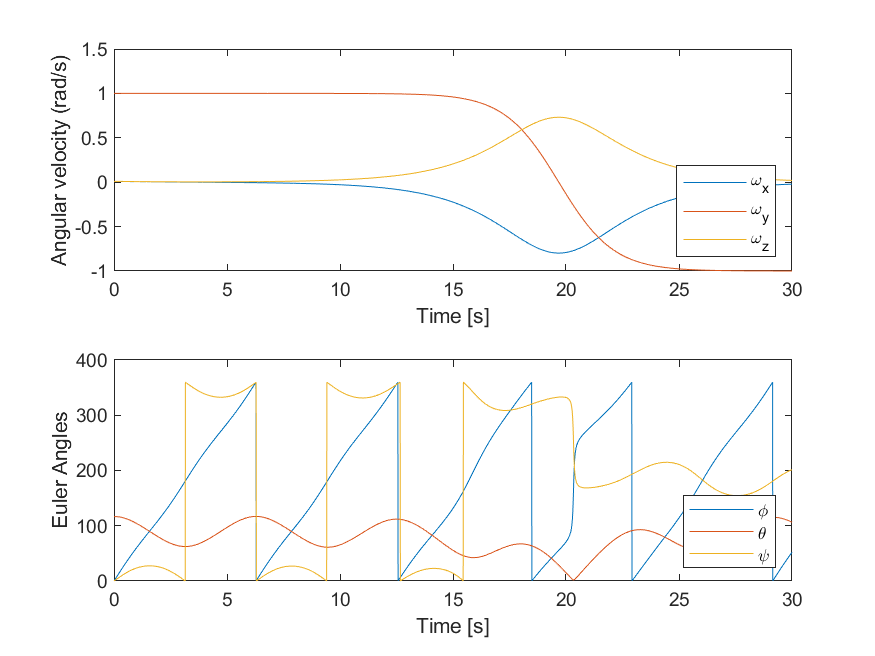
\includegraphics[scale=0.6]{Images/ps4_problem2a_2.png}
\caption{Simulation of satellite spinning on its intermediate principal axis}
\label{fig:ps4_problem2a_2}
\end{figure}

\begin{figure}[H]
\centering
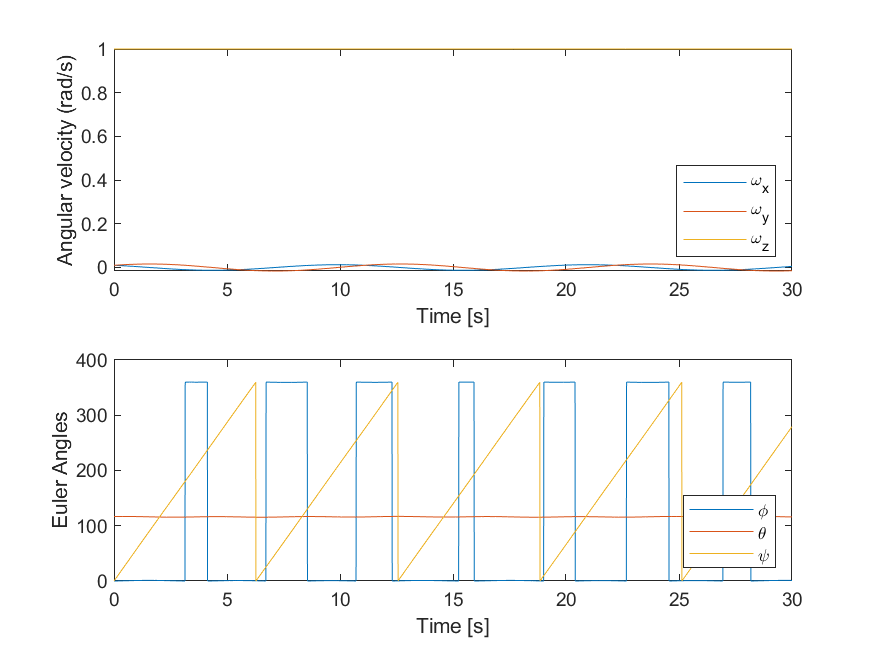
\includegraphics[scale=0.6]{Images/ps4_problem2a_3.png}
\caption{Simulation of satellite spinning on its maximum principal axis}
\label{fig:ps4_problem2a_3}
\end{figure}

\subsection{PROBLEM 3}
\textit{Adding a momentum wheel or rotor (dual-spin satellite)}

\textit{a. Re-program Euler equations to include a generic momentum wheel or rotor with rotation axis aligned with one of the principal axes of inertia. Ideally the wheel or rotor has specs representative of commercial products (inertia, rotational speed).}

The equations that implement the generic momentum wheel with the rotor into the Euler equations are below.

\begin{align*}
    I_x \dot{\omega_x} + I_r \dot{\omega_r} r_x + (I_z - I_y) \omega_y \omega_z 
    + I_r \omega_r (\omega_y r_z - \omega_z r_y) = M_x \\
    I_y \dot{\omega_y} + I_r \dot{\omega_r} r_y + (I_x - I_z) \omega_z \omega_x 
    + I_r \omega_r (\omega_z r_x - \omega_x r_z) = M_y \\
    I_z \dot{\omega_z} + I_r \dot{\omega_r} r_z + (I_y - I_x) \omega_x \omega_y 
    + I_r \omega_r (\omega_x r_y - \omega_y r_x) = M_z \\
    I_r \dot{\omega_r} = M_r
\end{align*}

The function kinEulerAngleWheel was used in addition to ode113 to simulate the angular velocities over time.

\textit{b. Numerically integrate Euler AND Kinematic equations from equilibrium initial condition. Verify that integration is correct as from previous tests (conservation laws, rotations, etc.).}

kinEulerAngleWheel was modified to also account for the kinematic equations, as shown before. As we see in Figure \ref{fig:ps4_problem3c_principal}, the overall momentum is conserved in the principal frame, as expected. Additionally, Figure \ref{fig:ps4_problem3c_inertial} shows that the angular momentum vector is conserved in the inertial frame, as expected.

\lstinputlisting{src/kinEulerAngleWheel.m}

\begin{figure}[H]
\centering
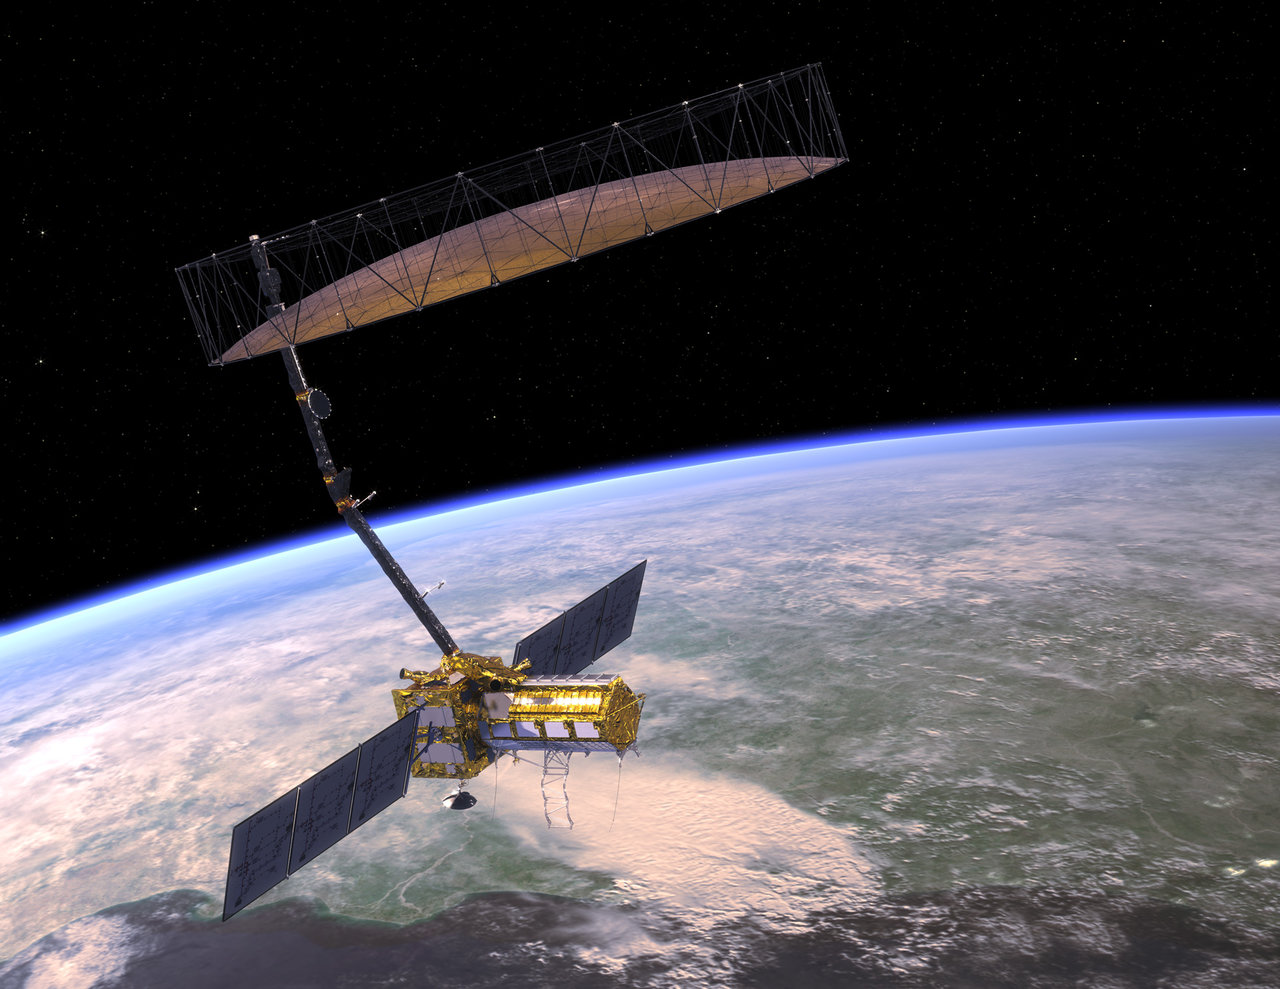
\includegraphics[scale=0.6]{Images/NISAR.jpg}
\caption{Angular Momentum in Principal Frame}
\label{fig:ps4_problem3c_principal}
\end{figure}

\begin{figure}[H]
\centering
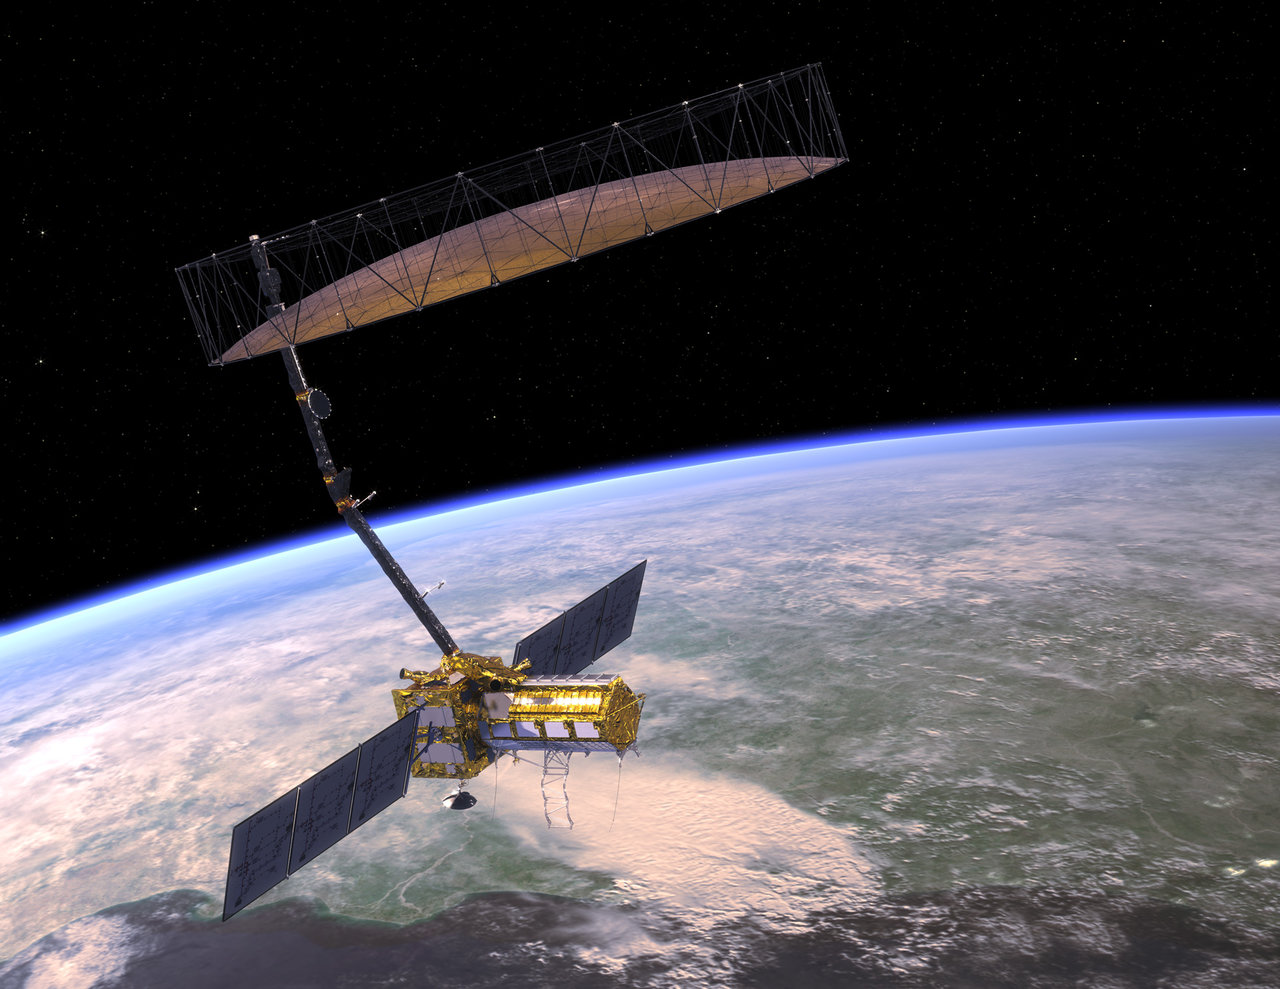
\includegraphics[scale=0.6]{Images/NISAR.jpg}
\caption{Angular Momentum in Inertial Frame}
\label{fig:ps4_problem3c_inertial}
\end{figure}

\textit{c. Verify equilibrium and its stability similar to previous pset.}

Based on linearizing the Euler equations around equilibrium, it can be found that periodic stability can be met with a reaction wheel if one of the following conditions are met:

\begin{align*}
    1)\; I_r \omega_r > (I_y - I_z) \omega_z \;\; AND \;\; I_r \omega_r > (I_x - I_z) \omega_z \\
    2)\; I_r \omega_r < (I_y - I_z) \omega_z \;\; AND \;\; I_r \omega_r < (I_x - I_z) \omega_z \\
\end{align*}

The above equation is specifically for equilibrium about the z-axis, but similar equations hold true for stability about the x and y axes.

Below are the angular velocity plots for stability about the maximum, intermediate, and minimum principal axes.

\textbf{figs}


\textit{d. Use the stability condition to make attitude motion stable for rotation about intermediate moment of inertia by changing moment of inertia and/or angular velocity of the momentum wheel or rotor.}




\textit{e. Try to make rotation about another arbitrary axis (potentially relevant to your project) stable through a generic momentum wheel or rotor.}

\subsection{PROBLEM 4}
\textit{Gravity gradient torque (modeling)}

\textit{a. Remove rotor.}

A new function was created without effect of the rotor.

\textit{b. Program gravity gradient torque. Feed torque to Euler equations. This is the first perturbation you model resulting from the interaction of the spacecraft with the environment. Hint: change your orbit to make gravity gradient significant if that’s not the case.}

The equations for the gravity gradient torque are below.

\begin{align*}
    I_x \dot{\omega_x} + (I_z - I_y) \omega_y \omega_z = 3 n^2 (I_z - I_y) c_y c_z \\
    I_y \dot{\omega_y} + (I_x - I_z) \omega_z \omega_x = 3 n^2 (I_x - I_z) c_z c_x \\
    I_z \dot{\omega_z} + (I_y - I_x) \omega_x \omega_y = 3 n^2 (I_y - I_x) c_x c_y \\
\end{align*}

In the above equation, $\Vec{c} = [cx, cy, cz]$ is the normalized direction of $\Vec{R}$.

The function gravGrad was developed to be used with ode113 to propagate the Euler equations.

\lstinputlisting{src/gravGrad.m}

\textit{c. Verify that the magnitude of the modeled torque is consistent with the orbit and inertia tensor of your satellite. Hint: use simplified formulas from class on modeling of gravity gradient torque.}

The general trends we would expect in the gradient gravity torque is for the value to be zero if the satellite spins on its normal axis at the mean motion and for the magnitude to grow linearly with the inertia tensor. The first property is demonstrated in Figure \textbf{fig1} and the second is demonstrated in Figure \textbf{fig2}.

Additionally, we can estimate the order of magnitude to expect our gravity gradient torques to be based on the below equation.

\begin{align*}
    \Vec{M} &= \frac{3 \mu}{a^3}
    \begin{bmatrix}
    (I_z - I_y) c_y c_z \\
    (I_x - I_z) c_z c_x \\
    (I_y - I_x) c_x c_y
    \end{bmatrix}
\end{align*}

The parameters used were the known moments of inertia ($I_x = \qty{7707}{}$, $I_y = \qty{14563}{}$, $I_z = \qty{18050}{\kilogram\cdot\meter^2}$), known values for Earth ($a = \qty{7125.49}{km}$, $\mu = \qty{398600}{\km^3\per\second^2}$), and an arbitrary $\Vec{c} = [\frac{1}{\sqrt{3}}, \frac{1}{\sqrt{3}}, \frac{1}{\sqrt{3}}]$. With these values, we get:

\begin{align*}
    \Vec{M} &=
\qty[parse-numbers = false]{
    \begin{bmatrix}
    0.384174 \\
    1.13956 \\
    -0.755387
    \end{bmatrix}
    \cdot
    10^{-2}
}{\newton\meter}
\end{align*}

These values are in line with what we see in Figure \textbf{fig}.

\textit{d. Numerically integrate Euler and Kinematic equations including gravity gradient from initial conditions corresponding to body axes aligned with the orbital frame (RTN). Verify that gravity gradient torque is zero, besides numerical errors. Hint: you may need to simplify the orbit to unperturbed circular to achieve this. Check that initial angular velocity matches mean motion.}

The constant gravity gradient was demonstrated in problem 4c in Figure \textbf{same fig as before}. Figure \textbf{fig3} demonstrated that the angular velocity in the normal direction matches the mean motion throughout the orbit.

\textit{e. Numerically integrate Euler and Kinematic equations including gravity gradient from arbitrary initial conditions (e.g., relevant to your project). Plot external torque (3 components w.r.t. time) and resulting attitude motion (depends on attitude parameterization, add Euler angles for better geometrical interpretation) over multiple orbits. Comment on results.}

fuck me with a shoe idk what to put here rn (will add later)